\documentclass[12pt]{article}
\usepackage{geometry}
\geometry{letterpaper}
\pdfoutput=1
\usepackage[pdftex]{graphicx}
\DeclareGraphicsExtensions{.png,.pdf,.eps}
\graphicspath{{./images/}}
\usepackage{float}
\usepackage{mathtools}
\usepackage{caption}
\usepackage{subcaption}
\usepackage{multirow}
\usepackage{amssymb}
\usepackage{authblk}

\title{Measuring the Higgs Self-Coupling Constant at a Multi-TeV Muon Collider}
%\author{
	%Alexander Conway\\
	%Department of Physics\\
	%The University of Chicago
	%and\\
	%Hans Wenzel\\
	%Computing Division\\
	%Fermi National Accelerator Laboratory\\
	%\\
	%Faculty Adviser: Dr.\ Young-Kee Kim\\
	%The University of Chicago}
\author[1]{Alexander Conway\thanks{aconway@fnal.gov}}
\author[2]{Hans Wenzel}
\author[2]{Estia Eichten}
\author[2]{Ronald Lipton}

\affil[1]{The University of Chicago\\ 
Faculty Adviser: Young-Kee Kim}
\affil[2]{Fermi National Accelerator Laboratory}

\date{\today}

\begin{document}
\maketitle

\begin{abstract}
	A lepton collider in the multi-TeV range has the potential to measure the trilinear Higgs self-coupling constant $\lambda_{hhh}$ via the W-fusion mode $\ell^+\ell^- \rightarrow \nu_\ell \bar{\nu}_\ell h h$. In this paper we do a generator-level study to explore how center-of-mass energy spread, cone size, tracking resolution, and collision energy range affect how precisely a muon collider can measure $\lambda_{hhh}$ in comparison to an $e^+e^-$ collider. The smaller spread in center-of-mass energy and higher energy range of a muon collider improve cross section while the larger cone required to reduce beam-induced background hinders detection of double-Higgs events. Our results motivate a more detailed study of a multi-TeV muon collider and innovative detector and analysis technologies required for background rejection and precision measurement.
\end{abstract}

\section{Introduction}
Measurement of the Higgs trilinear self-coupling is a direct probe of the shape of the Higgs potential and a crucial test of the Standard Model. In the Standard Model, the Higgs potential is given by Eq.~\ref{eq:h-pot}:

\begin{equation}
	V(\eta_h) = \frac{1}{2}m_h^2\eta_h^2 + \lambda_{hhh}\nu\eta_h^3 + \frac{1}{4}\lambda_{hhhh}\eta_h^4 \label{eq:h-pot}
\end{equation}

The trilinear self-coupling is defined in the Standard Model as $\lambda_{hhh} = \lambda_{hhhh}= (m_h^2/2v^2) \approx 0.13$ for Higgs mass $m_h = 125~GeV$ and vacuum expectation value $v = {(\sqrt{2}G_F)}^{-1/2} \approx 246~GeV$~\cite{goertz}. For convenience we will use $\lambda = \lambda_{hhh}$ to refer to the measured value and $\lambda_{SM}$ to refer to the value predicted by the Standard Model.

\begin{figure}[h]
	\centering
	\begin{subfigure}[b]{0.3\textwidth}
		\centering
		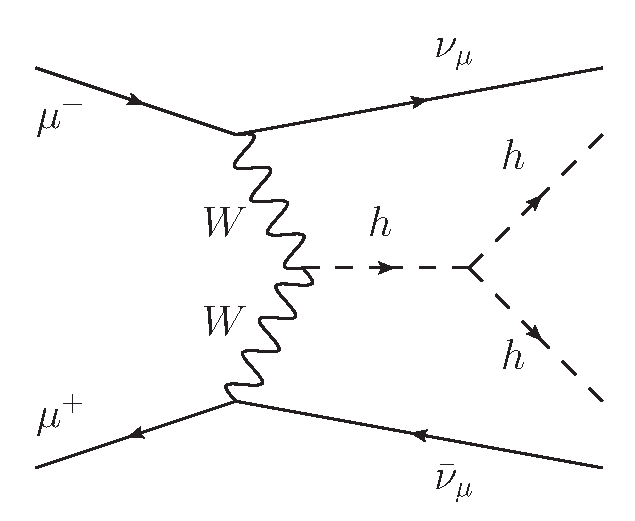
\includegraphics[width=0.9\textwidth]{diagram-trilin}
		\caption{}\label{subfig:diagram-trilin}
	\end{subfigure}
	\begin{subfigure}[b]{0.3\textwidth}
		\centering
		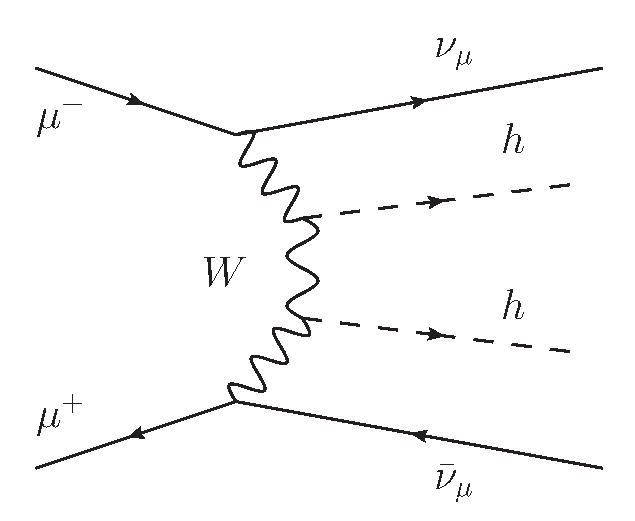
\includegraphics[width=0.9\textwidth]{diagram-radiation}
		\caption{}\label{subfig:diagram-radiation}
	\end{subfigure}
	\begin{subfigure}[b]{0.3\textwidth}
		\centering
		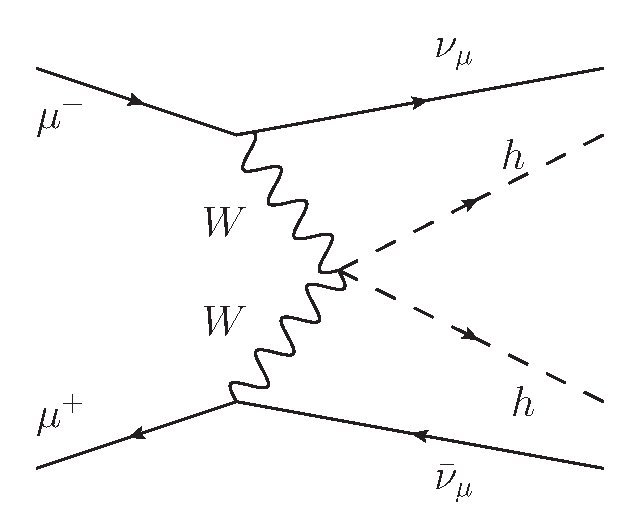
\includegraphics[width=0.9\textwidth]{diagram-4x}
		\caption{}\label{subfig:diagram-4x}
	\end{subfigure}
	\caption{Feynman diagrams of the three double-Higgs production modes accessible at a multi-TeV muon collider. Figure~\ref{subfig:diagram-trilin} is the only process directly affected by the value of $\lambda$ but interference between these diagrams means each contributes to the Higgs self-coupling measurement.}\label{fig:feyn-diags}
\end{figure}

Figure~\ref{fig:feyn-diags} shows the three processes at a muon collider whose cross sections are affected by the value of the trilinear Higgs self-coupling. Only the diagram in Figure~\ref{subfig:diagram-trilin} is directly affected by the value of $\lambda$, but the total cross section of all three processes contributes to the measurement because interference between them affects their cross sections.

It is estimated that with an integrated luminosity of $3000~fb^{-1}$, the LHC will be able to measure $\lambda$ with an uncertainty of $\sim + 30 \%$ and $\sim - 20 \%$~\cite{goertz}. This measurement has been studied for $e^+e^-$ colliders and it is anticipated that a machine such as the proposed $e^+e^-$ Compact Linear Collider (CLIC) could reduce uncertainties to as low as $\pm 11\%$~\cite{pres:jan}. A muon collider should ostensibly have very similar signal physics and background properties because we assume lepton universality, meaning that muons and electrons couple equally to W and Z bosons. However, differences in beam and detector properties lead to differences that affect this measurement at each potential machine. 

The trilinear Higgs self-coupling measurement has been extensively studied for CLIC~\cite{clic-physics,pres:jan}. The basic method is to measure the cross section of double-Higgs production events and compare it to values predicted for varying values of $\lambda$. In addition some studies perform template fits to the distribution of the decay angle, which is sensitive to $\lambda$ because the relative dominance of the three different signal processes leads to different kinematics~\cite{clic-physics}. The cross section is measured using an Artificial Neural Network (ANN) to tag double-Higgs events based on jet tags, kinematics, and other predictors~\cite{pres:jan}. 

Research and development for the muon collider is not yet at the stage where a comparably detailed study is possible; detector and shielding designs, full background simulations, and reconstruction methods are still in early development. We present here a brief study of key aspects of a muon collider which differentiate its ability to measure this constant from that of an $e^+e^-$ collider using generator-level simulation and parametrized detector acceptance to describe the physics signal. CLIC design reports serve as a basis for comparison of cone angles and signal properties~\cite{clic-physics,pres:jan}. Parameters for the muon collider are taken from the 2013 Snowmass Whitepaper from the U.S. Muon Accelerator Program (MAP)~\cite{usmap}. In particular we study the impacts of a more narrow center-of-mass energy spread, the higher energy range of a muon collider, different tracker geometries, and the larger shielding cone needed for the reduction of beam-induced background. 

\section{Generator Level Studies}
We use \textsc{Whizard 2} with O'Mega~\cite{whizard,omega} to calculate cross sections, \textsc{MadGraph 5}~\cite{madgraph} with a \textsc{Pythia 6.4}~\cite{pythia} interface for event generation and hadronization, and org.lcsim~\cite{lcsim} for analysis. We assume a Standard Model Higgs boson with mass $M_h = 125\ GeV$ and total width $\Gamma_h = 4.07\ MeV$ with the exception of modifying the value of $\lambda$.

We compare our data to CLIC studies using an $e^+e^-$ beam with center of mass energy $\sqrt{\hat{s}}=3~TeV$ and unpolarized beams. These studies used a Standard Model Higgs with mass $M_h=120~GeV$, which slightly increases the cross section of the double-Higgs production modes. Note that beam polarization at an $e^+e^-$ machine may increase the double-Higgs production cross section by a factor of up to two~\cite{pres:jan}.

To compare the two machines we assume the acceptance of $\ell^+\ell^- \rightarrow \nu_\ell \bar{\nu}_\ell hh \rightarrow b\bar{b}b\bar{b}$ events for each detector geometry is representative of the relative efficiencies for all double-Higgs events. Then we use the different acceptances, luminosities, and cross sections to compare the expected number of double-Higgs and background events to compute the estimated uncertainty in the self-coupling measurement, using the assumption that background rejection and physics signatures will be effectively identical between the two machines.

\subsection{Cross Sections and Luminosity}
\subsubsection{Cross Sections}
In first order, the signal and physics backgrounds at a multi-TeV muon collider are identical to those at an electron collider. However, the wider spread in collision energies at an electron collider reduces the cross section at $\sqrt{\hat{s}}=3~TeV$ by about $27\%$, whereas the energy spread for a muon collider in this range is negligible. Additionally, the muon collider can operate at $\sqrt{\hat{s}}=6~TeV$ and potentially beyond, increasing the cross section by a factor of $2.4$ at the cost of more forward events. Figure~\ref{fig:xsects} illustrates the difference in cross section between $e^+e^-$ and $\mu^+\mu^-$ machines. 

\begin{figure}
	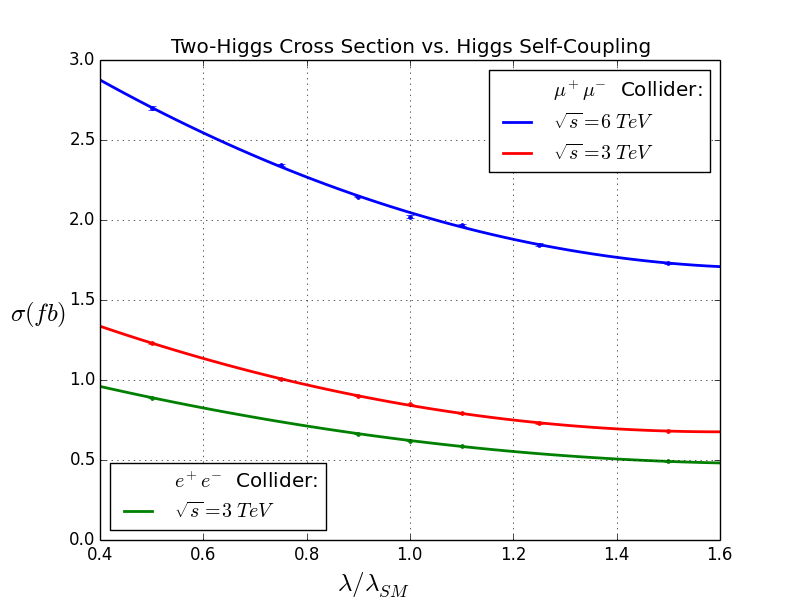
\includegraphics[width=\textwidth]{xsects}
	\caption{Comparison of double-Higgs production cross sections at lepton colliders. The lower cross section for electron-positron collider at the same nominal center-of-mass energy is due to its higher center-of-mass energy spread, caused by initial state radiation and beam-beam effects. This is believed to be negligible for a muon collider. The data are fitted to a parabola. Muon collider calculations done with \textsc{Whizard 2},~\cite{whizard,omega}}\label{fig:xsects} $e^+e^-$ data is taken from~\cite{pres:jan}.
\end{figure}

The sensitivity of the cross section to the value of $\lambda/\lambda_{SM}$ is used to convert  from measured cross section uncertainty to the self-coupling measurement uncertainty as shown in Equation~\ref{eq:sigtolam}.

\begin{equation}
	\frac{\delta\lambda}{\lambda_{SM}} = R \frac{\delta\sigma}{\sigma}\label{eq:sigtolam}
\end{equation}
where
\begin{equation}
	R \equiv \left.\frac{\delta\lambda/\lambda} {\delta \sigma/\sigma}\right|_{\substack{\lambda=1 \\ \sigma=\sigma_{meas}}}\label{eq:defR}
\end{equation}

and the derivatives in Eq.~\ref{eq:defR} are calculated by fitting the cross section vs $\lambda/\lambda_{SM}$ curves in Figure~\ref{fig:xsects} to a parabola. The values of R for each machine, assuming Standard Model cross sections, are found in Table~\ref{table:Rs}.

\begin{table}
	\centering
	\begin{tabular}{|c | c | c|}
		\hline
		\multirow{2}{*}{$\sqrt{\hat{s}}$}	& \multicolumn{2}{|c|}{$R$} \\
		\cline{2-3}
		& CLIC	& Muon Collider \\ \hline
		$3~TeV$	& 1.52	& 1.53 \\ \hline
		$6~TeV$	& ---	& 2.08 \\ \hline
	\end{tabular}
	\caption{Scaling factors for propagating uncertainty from $\delta \sigma/\sigma$ to $\delta \lambda/\lambda_{SM}$.}\label{table:Rs}
\end{table}

\subsubsection{Luminosity}

\begin{table}
	\centering
	\begin{tabular}{|c | c | c|}
		\hline
		\multirow{2}{*}{$\sqrt{\hat{s}}$}	& \multicolumn{2}{|c|}{$\mathcal{L}~(10^{34}cm^{-2}s^{-1})$} \\
		\cline{2-3}
		& CLIC	& Muon Collider \\ \hline
		$3~TeV$	& 5.4	& 4.4 \\ \hline
		$6~TeV$	& ---	& 12 \\ \hline
	\end{tabular}
	\caption{Expected luminosities at CLIC and a Muon Collider~\cite{clic-physics,usmap}.}\label{table:Ls}
\end{table}

The expected average luminosities for CLIC and the Muon Collider are listed in Table~\ref{table:Ls}. The higher $3~TeV$ lumonisity at CLIC suggests that it will have better statistics than a Muon Collider at that energy, despite the slightly lower cross section. Figure~\ref{fig:num-higgs} compares the expected total numbers of double-Higgs events at each machine after 5 `Snowmass years', or $5\times10^7s$.

\begin{figure}
	\centering
	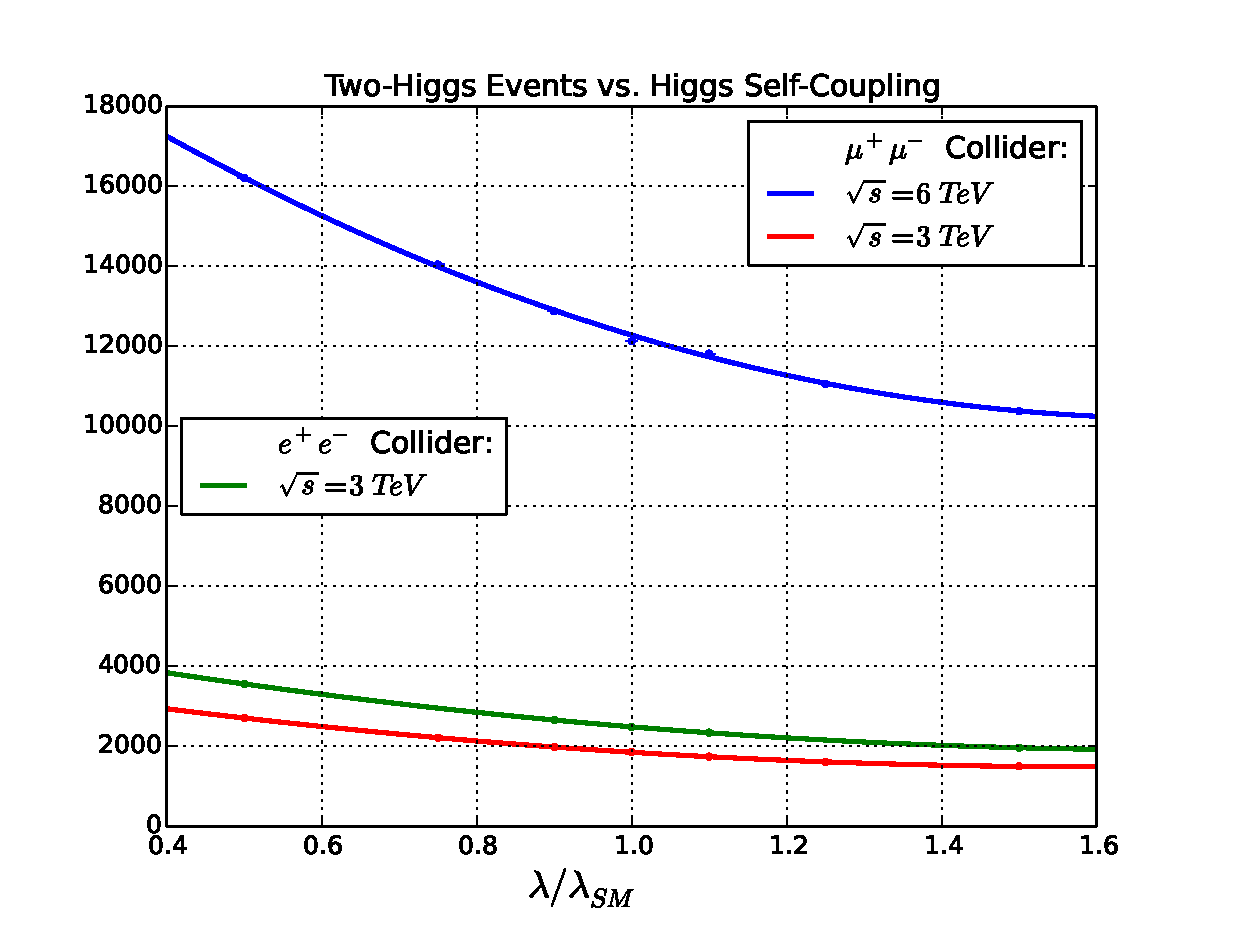
\includegraphics[width=\textwidth]{num_higgs}
	\caption{Estimated number of double-Higgs events after five Snowmass years, or $5\times10^7s$.}\label{fig:num-higgs}
\end{figure}

%\subsection{Decay Angle}

%\begin{figure}
	%\centering
	%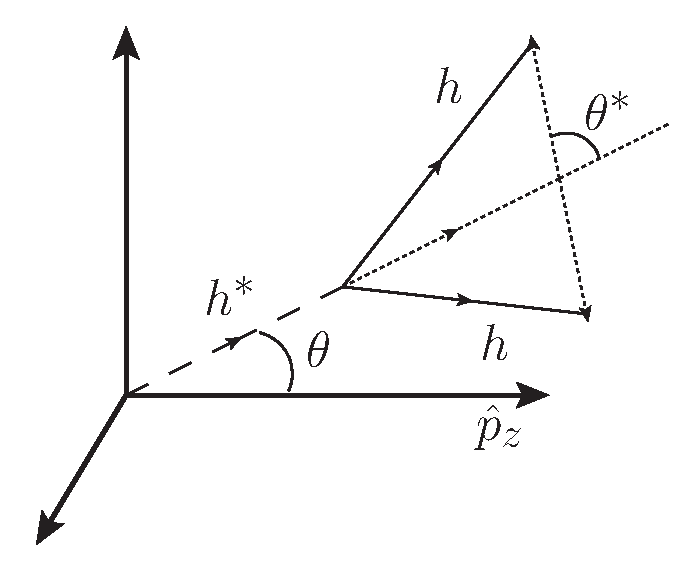
\includegraphics[width=0.6\textwidth]{decay-angle}
	%\caption{Diagram illustrating the definition and measurement of the decay angle $\theta^*$, the angle of the decay products with respect to the boost direction in the two-Higgs rest frame.}\label{fig:decay-angle}
%\end{figure}

%For a boosted decay to two equally massive particles there is a decay angle $\theta^*$ which describes the angle between the decay products and the direction of boost in the boosted frame, as seen in Figure~\ref{fig:decay-angle}. The decay angle is calculated with Equation (\ref{eq:decay-angle}):

%\begin{equation}
	%\cos\theta^* = 4 \frac{(\vec{p}_{h_1} - \vec{p}_{h_2}) \cdot (\vec{p}_{h_1} + \vec{p}_{h_2})} {|(\vec{p}_{h_1} - \vec{p}_{h_2})| |(\vec{p}_{h_1} + \vec{p}_{h_2})|}\label{eq:decay-angle}
%\end{equation}

%The distribution of $\lvert\cos\theta^*\rvert$ is sensitive to the value of $\lambda_{hhh}$ because the three processes (Figure~\ref{fig:feyn-diags}) have different kinematics, as can be seen in Figure~\ref{fig:cos-thetastar}. Therefore this distribution can be used as an ANN input to tag double-Higgs decays and calculate the cross section or be used in a maximum-likelihood template fit along with other measured parameters.

%\begin{figure}
	%\centering
	%\begin{subfigure}[b]{0.8\textwidth}
		%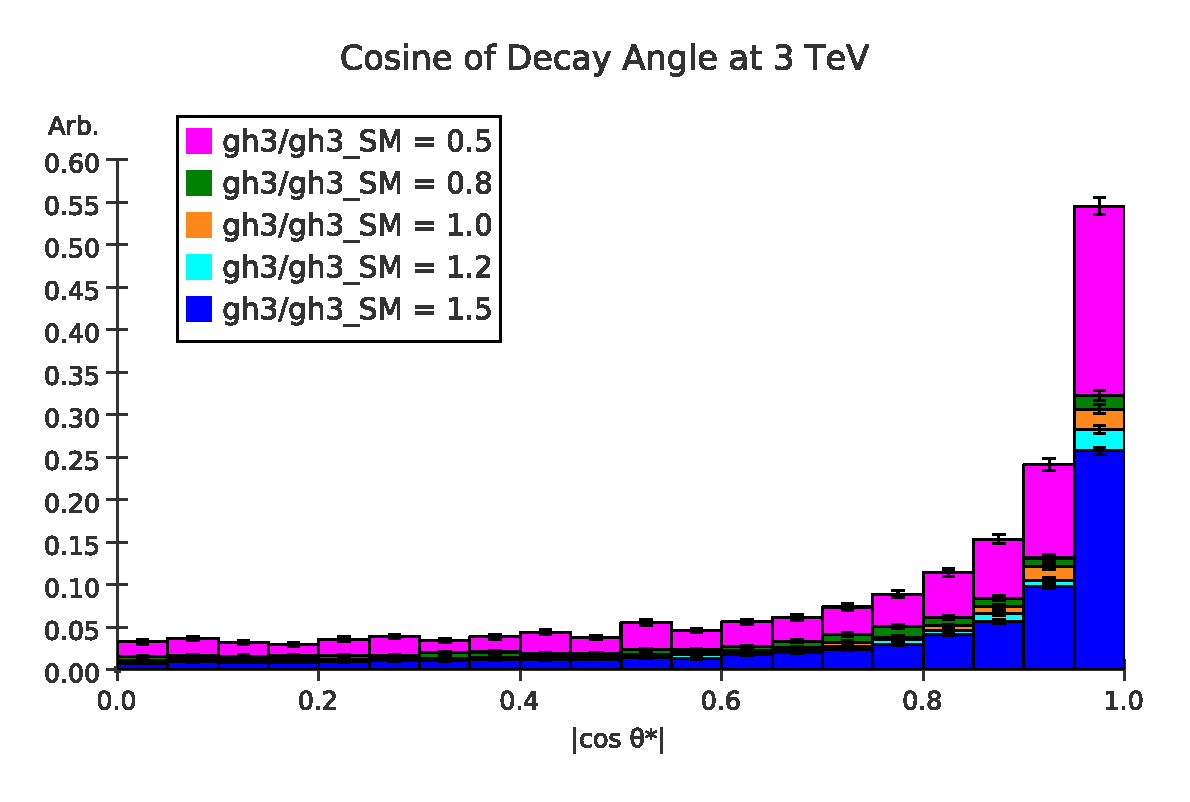
\includegraphics[width=\textwidth]{cos-thetastar-3tev}
		%\caption{}\label{subfig:cos-thetastar-3tev}
	%\end{subfigure}
	%\begin{subfigure}[b]{0.8\textwidth}
		%\centering
		%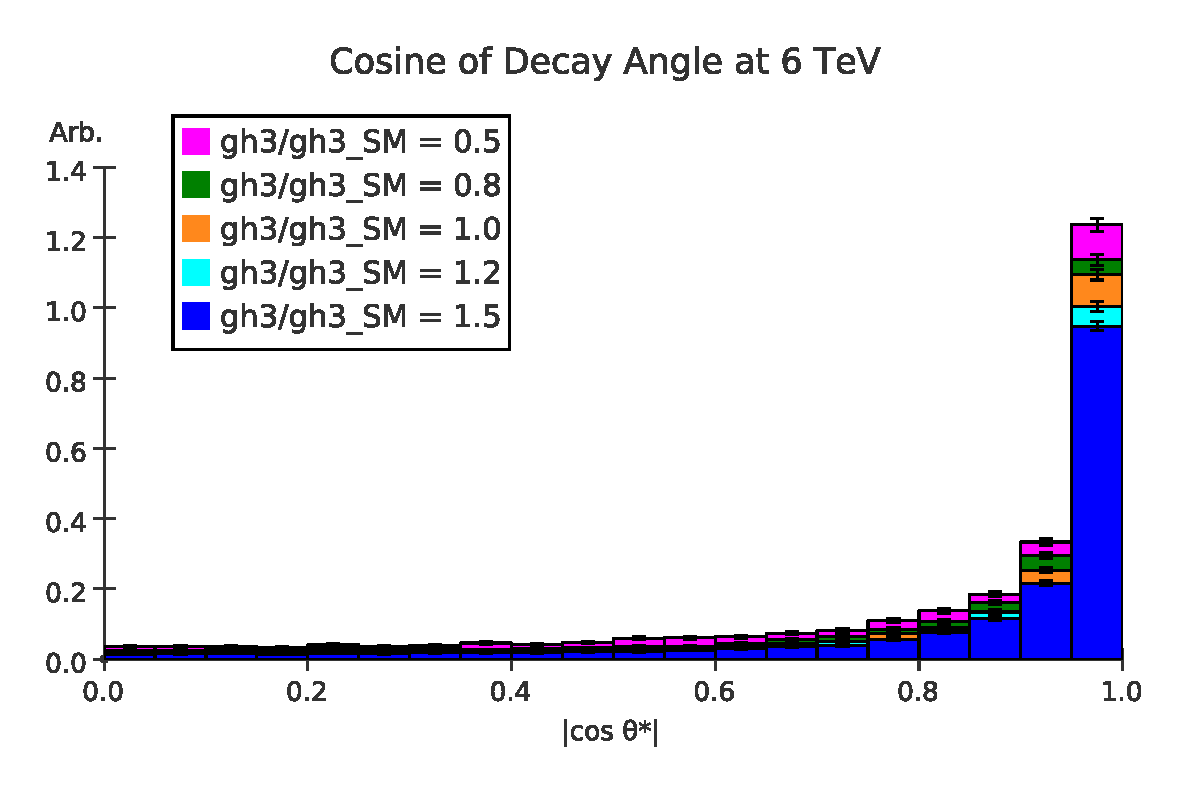
\includegraphics[width=\textwidth]{cos-thetastar-6tev}
		%\caption{}\label{subfig:cos-thetastar-6tev}
	%\end{subfigure}
	%\caption{$\lvert\cos\theta^*\rvert$ distributions at $3~TeV$ $(6~TeV)$ for various values of $\lambda/\lambda_{SM}$, weighted by cross section. Statistics correspond to roughly $11000~fb^{-1}$ $(5000~fb^{-1})$, or $10,000$ events.}\label{fig:cos-thetastar}
%\end{figure}

\subsection{Detector Geometry}
A muon collider requires a detector with good suppression of the beam-induced background. This will be accomplished by increasing the angle of the beam pipe cone, reducing forward tracking coverage, and by using more radiation-hard materials in the tracking system, reducing tracking precision. We compare propsed detector geometries for CLIC and a muon collider in their ability to observe double-Higgs events, focusing on the $hh\rightarrow b\bar{b}b\bar{b}$ channel in particular.

%One potential disadvantage of a muon collider in comparison to an electron-positron collider is the larger beam pipe cone required for detector shielding. CLIC could potentially have effective tracking up to $\sim7^{\circ}$ from the beam axis~\cite{clic-physics} while estimates for the muon collider cone are $\sim15^{\circ}$ for a Higgs factory machine and $\sim10^{\circ}$ for a high-energy machine. Beam-induced backgrounds at a muon collider decrease with increased center-of-mass energy, so higher-energy machines will require smaller cones. To quantify the effect of the cone size on the two-Higgs signal we model the cone as a simple linear cone extending from the vertex and assume that we cannot detect any particles with momentum vectors pointing into the cone and can detect all other particles (barring neutrinos). 

\subsubsection{Visible Energy}
We define `visible energy' as the total energy theoretically visible to the detector; it is the sum of the energies of all final state particles with momentum vectors that don't point into the cone, barring neutrinos. As a simple exercise to estimate the effect of the cone on the signal we simulated double-Higgs production events with $\lambda=\lambda_{SM}$ at center-of-mass energies $\sqrt{\hat{s}} = 3\ TeV$ and $6\ TeV$ and recorded the total visible energy as a fraction of the energy visible with no cone for a range of cone angles, as seen in Figure~\ref{fig:visen}. We find that a cone angle of $10^{\circ}$ blocks approximately half of the energy in the signal events at $3\ TeV$ and up to two thirds at $6\ TeV$. The tradeoff between more forward events versus higher cross sections and smaller cones at higher energies will need to be studied in greater detail.

\begin{figure}
	\centering
	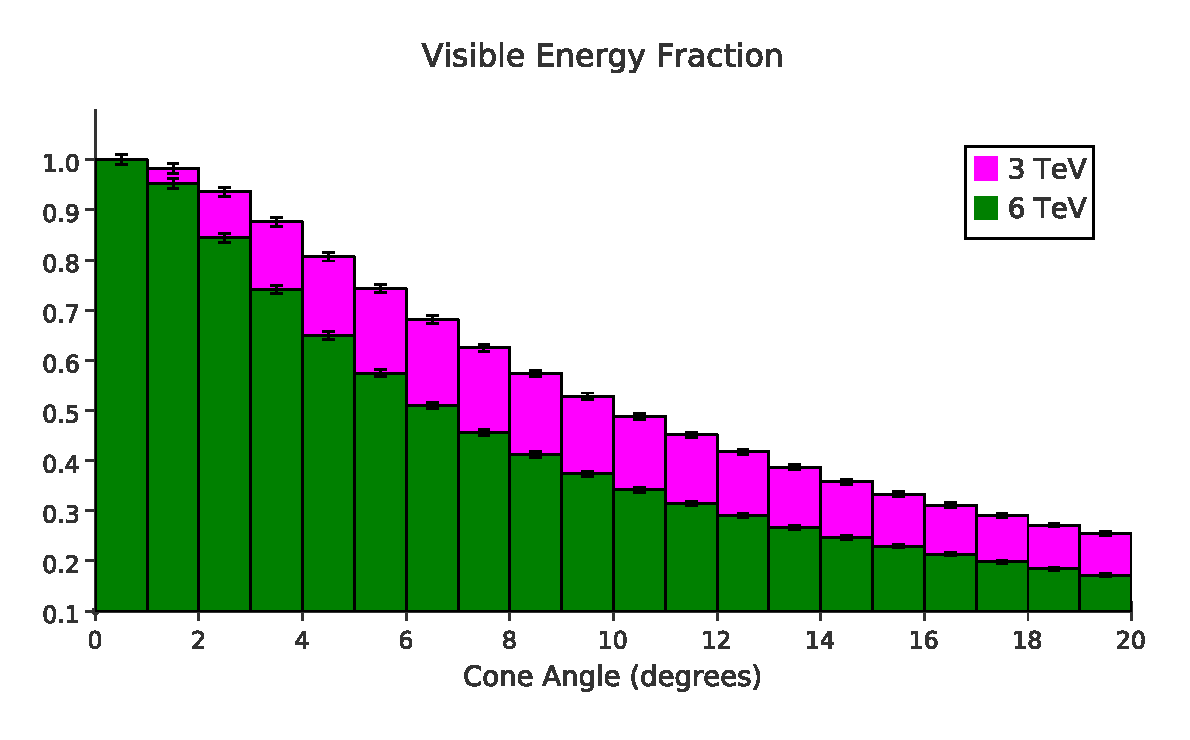
\includegraphics[width=0.8\textwidth]{visen}
	\caption{Fraction of energy visible to a detector with given cone angles in double-Higgs production events with $\lambda=\lambda_{SM}$. Events generated by \textsc{Whizard 2}~\cite{whizard} and hadronized with \textsc{Pythia 6.4}~\cite{pythia}}\label{fig:visen}
\end{figure}

\subsubsection{b-Tagging}
Visible energy does not tell the whole story and it's important to look at the specifics of certain Higgs decay channels, particularly events where both Higgs bosons decay into $b\bar{b}$ pairs. This is the largest single channel in the signal, making up about $33\%$ of the double-Higgs events for a Standard Model $125\ GeV$ Higgs. The cross section is therefore $0.28fb$, without any kinematic cuts, and the four-$b$ physics background to this is $\sim4fb$ at $3\ TeV$. This background becomes orders of magnitude larger when fake rates and jet-clustering effects are considered.

We use the four-$b$ channel to test the effects of cone angle and track resolution on the ability to tag all four $b$'s in a double-Higgs event. We define a $b$ quark as taggable if it has a displaced vertex outside the cone and produces least two charged particle tracks with significant three-dimensional impact parameters. Impact parameters are significant if they are at least three times larger than their measured uncertainty. We simulated double-Higgs to $b\bar{b}$ pairs in \textsc{MadGraph 5} and hadronized them in \textsc{Pythia}. Track reconstruction and parameter calculation was carried out using the `MCFast()' org.lcsim driver and geometry files for the CLIC `sidloi3' detector~\cite{sidloi3}. We then calculated the fraction of signal events with four taggable $b$'s to get the effective acceptance, as seen in Figure~\ref{fig:cone-xsects}.

\begin{figure}
	\centering
	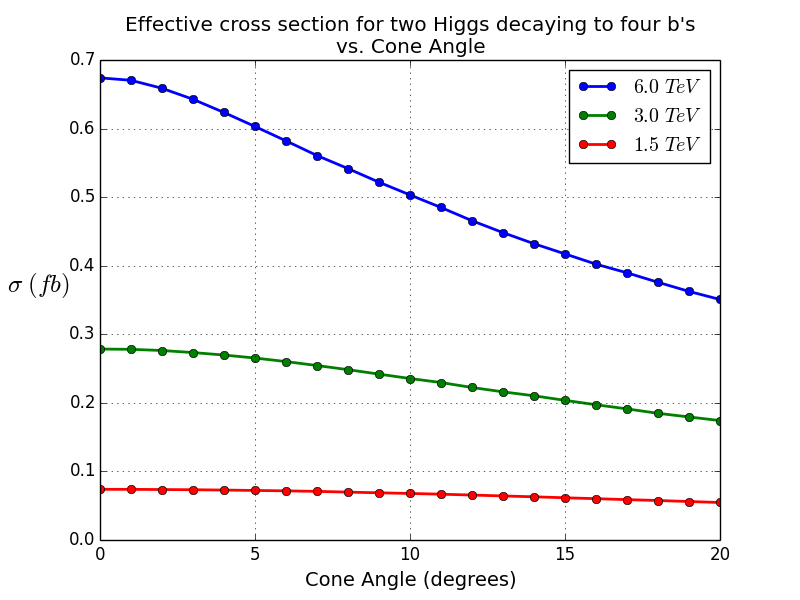
\includegraphics[width=0.8\textwidth]{cone_xsects}
	\caption{Effective cross sections of $hh\rightarrow b\bar{b}b\bar{b}$ signal events where we require that all four $b$'s can theoretically be tagged. This is calculated as $\sigma(\mu^+\mu^-\rightarrow \nu_\mu \bar{\nu}_\mu h h) \times Br{(h\rightarrow b\bar{b})}^2 \times \epsilon_{acc}$ where $\epsilon_{acc}$ is the acceptance rate for four-$b$ signal events. The acceptance rate is calculated by assuming events with four `taggable' $b$'s. A $b$ is `taggable' if it has a displaced vertex outside the cone and produces least two charged particle tracks with significant three-dimensional impact parameters.}\label{fig:cone-xsects}
\end{figure}

%We find that a cone angle of $10^{\circ}$ has a $13\%$ effect on four-$b$ acceptance at $1.5\ TeV$, $17\%$ at $3\ TeV$ and $26\%$ at $6\ TeV$. In this particular regard a $\mu^+\mu^-$ collider is comparable to an $e^+e^-$ collider.

%At $3~TeV$ we find four-$b$ acceptances of $90\%$ and $83\%$ with $7^\circ$ and $10^\circ$ cones, respectively. For 5 Snowmass years of data we calculate that the theoretical limit of the $hh\rightarrow b\bar{b}b\bar{b}$ channel sensitivity to $\frac{\Delta\lambda/\lambda_{SM}}{\lambda/\lambda_{SM}}$ is $2.5\%$ at CLIC and $1.8\%$ at the Muon Collider. This physics channel will be accessible at a $6~TeV$ Muon Collider and may provide the opportunity for an even more precise measurement.


\section{Conclusions and Remarks}
A muon collider presents distinct advantages and disadvantages for a precise measurement of the trilinear Higgs self-coupling. The higher signal cross section at a $3TeV$ Muon Collider compared to CLIC increases the cross section and sensitivity, but the higher luminosity at CLIC provides more statistics. The cones required for shielding pose a significant challenge due to the amount of energy they block and the forward-boosted nature of the signal events. Our analysis of the 4-$b$ channel suggests that the increased cross section of the physics signal at a $6~TeV$ Muon Collider outweighs the signal lost in the cone due to the increased forward boost. There are also other factors that have yet to be studied in detail, particularly machine-induced backgrounds. Our results suggest that a muon collider has the potential to measure $\lambda_{hhh}$ as well as or better than an electron-positron collider with a sufficiently advanced detector. Further research and development of accelerator, detector, and analysis technologies and in-depth study of the physics opportunities at a multi-TeV muon collider will be necessary to fully determine the project's feasability.

\subsection{Acknowledgments}
The authors would like to thank Jan Strube and Heather Logan for their support and collaboration. Operated by Fermi Research Alliance, LLC under Contract No. De-AC02-07CH11359 with the United States Department of Energy.

\bibliographystyle{plain}
\bibliography{bib/writeup}

\end{document}
